\documentclass[12pt]{article}
\usepackage[a4paper, total={7.5in, 11in}]{geometry}
\usepackage{array}
\usepackage{graphicx, subfig, wrapfig, fancyhdr, lastpage, multicol ,color,arydshln,makecell}

\newcommand\headerMe[2]{\noindent{}#1\hfill#2}
\usepackage[mathscr]{euscript}
\usepackage{tabularray}

\setlength{\columnseprule}{1pt}
\def\columnseprulecolor{\color{blue}}


\pagestyle{fancy}
\fancyhf{}

\cfoot{ \vspace{-0.8cm}\em{Page \thepage \hspace{1pt} / \pageref{LastPage}}}
\begin{document}

\headerMe{Royaume du Maroc}{année scolaire \emph{2022-2023}}\\
\headerMe{Ministère de l'Éducation nationale, }{  Professeur :\emph{Zakaria Haouzan}}\\
\headerMe{du Préscolaire et des Sports}{Établissement : \emph{Lycée SKHOR qualifiant}}\\
%\vspace{-1cm}
\begin{center}
Devoir Surveillé  N°3 - S1 \\
    2ème année baccalauréat Sciences physiques\\
Durée 2h00
\\
    \vspace{.2cm}
\hrulefill
\Large{Chimie 7pts - 45min}
\hrulefill\\

    %\emph{Les deux parties sont indépendantes}
\end{center}
%end Headerss------------------------
%__________________Chimie ______________________-
%%%%%%%+_+_+_+_+_+_+_+_+_Partie1

 \section*{Partie 1 : Etude d’une solution aqueuse d’un acide carboxylique\dotfill(7pts)-45min }
%\begin{wrapfigure}{r}{0.16\textwidth}
	%\vspace{-1.2cm}
%%\begin{center}
  %%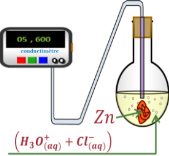
\includegraphics[width=0.16\textwidth]{./img/chimie01.png}
%%\end{center}
%\end{wrapfigure}


\begin{wrapfigure}[12]{r}{0.38\textwidth}
	\vspace{-2.4cm}
\begin{center}
  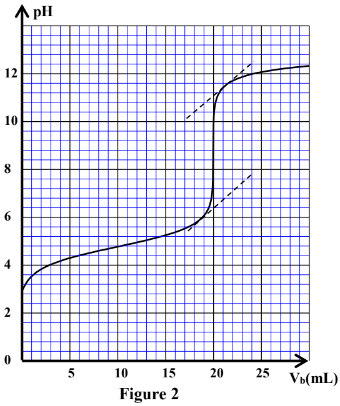
\includegraphics[width=0.38\textwidth]{./img/img00.png}
\end{center}
\end{wrapfigure}

Un flacon, dont l’étiquette est illisible, contient une solution aqueuse
Sa
d’un acide carboxylique de

formule et de concentration inconnues. Cette partie de l’exercice se propose :
\begin{itemize}
	\item  de déterminer la concentration de cette solution aqueuse.
	\item  d’identifier cet acide.
\end{itemize}
On notera AH pour désigner l’acide carboxylique et $A^-$
pour désigner sa base conjuguée.
Toutes les mesures sont réalisées à 25°C.

\hspace{-1cm} \textbf{1. Dosage de l’acide carboxylique\dotfill}

On dose un volume $V_a = 20 mL$ de la solution aqueuse
$S_a$ de concentration $C_a$ par une solution aqueuse $S_b$ d’hydroxyde de sodium $(Na^+_{(aq)} HO^-_{(aq)})$ de concentration $C_b = 10^{-1}mol.L^{-1}$
La courbe de la figure 2 représente les variations du pH
du mélange réactionnel en fonction du volume $V_b$ de la
solution basique versée.

	\begin{tabular}{c | c}
		1 & \makecell[l]{\textbf{1. }Ecrire l’équation de la réaction du dosage.}\\

		1 & \makecell[l]{\textbf{2. }Déterminer graphiquement les coordonnées $pH_E$ et $V_{bE}$ du point d’équivalence.}\\

			1 & \makecell[l]{\textbf{3. }Déterminer la valeur de la concentration $C_a$. }\\

	
						\end{tabular}
			
						\hspace{-1cm}\textbf{2. Identification de l’acide carboxylique\dotfill}

						La solution $S_a$ est préparée par dissolution de l’acide AH dans l’eau. La mesure du pH de la solution
Sa donne : $pH= 2,88$.

\begin{tabular}{c|l}
	1  & \makecell[l]{ \textbf{2.1. }Écrire l’équation chimique modélisant la réaction de l’acide propanoïque avec l’eau.}\\

	1	 & \makecell[l]{\textbf{2.2. }Montrer que le taux d’avancement final de la réaction est : $\tau \approx 1,32 \%$ }\\

	1 & \makecell[l]{\textbf{2.3. }Déterminer l’expression du quotient de la réaction $Q_{r,eq}$ à l’équilibre en fonction de $C_a$ et $\tau$.\\Vérifier que sa valeur est : $Q_{r,eq} \approx 1,77.10^{-5}$.}\\

	0,5 & \makecell[l]{\textbf{2.4. }Identifier l’acide carboxylique AH étudié en vous aidant du tableau des valeurs de $pK_A$ des\\
couples acide/base ci-dessous. Justifier votre réponse. }\\
\end{tabular}

\begin{center}
\begin{tabular}{ |c| c|}
\hline
\textbf{Couple acide/base} &\textbf{ Valeur de $pK_A$}\\\hline
	$HCOOH / HCOO^-$  & 3,75 \\\hline
	$C_6H_5COOH/C_6H_5COO^-$ &4,2\\\hline
	$CH_3COOH/CH_3COO^-$&  4,75 \\\hline
	$CH_3-CH_2-COOH/CH_3-CH_2-COO^-$ &4,9 \\\hline

\end{tabular}
\end{center}

\begin{tabular}{c|l}
	0,5 & \makecell[l]{\textbf{3. }Déterminer le volume
	$V_{b1}$ de la solution $S_b$ versée, au cours du dosage, pour que: $\frac{[AH]}{[A^-]} = 2,24$ . }\\
\end{tabular}

%\hrulefill
%\Large{Physique 13pts/78min}
%\hrulefill\\
\newpage
\begin{center}
    %\vspace{.60cm}
\hrulefill
\Large{Physique 13pts - 75min}
\hrulefill\\
    \emph{Les  parties sont indépendantes}
\end{center}

%\vspace{-1cm}
\section*{Partie 1 : Vérification de la capacité d'un condensateur C \dotfill(6,25pts)}

\begin{wrapfigure}[9]{r}{0.25\textwidth}
  \begin{center}
	  \vspace{-1cm}
	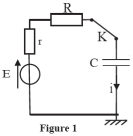
\includegraphics[width=0.19\textwidth]{./img/img01.png}
	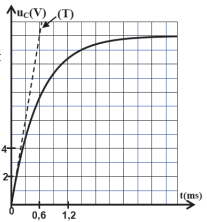
\includegraphics[width=0.25\textwidth]{./img/img02.png}
  \end{center}
\end{wrapfigure}
On réalise le circuit électrique schématisé
sur la figure 1 qui comporte :
\begin{itemize}
\item Un générateur de tension de f.e.m. (E).
\item  Deux conducteurs ohmiques de
résistance $r =20\Omega$ et R .
\item Un condensateur de capacité C
initialement déchargé .
\item Un interrupteur K à double position.
\end{itemize}
A un instant de date $t =0$, on place l’interrupteur K en
position (1). Un système d’acquisition informatisé permet de
tracer la courbe d’évolution de la tension $u_C(t)$. La droite (T)
représente la tangente à la courbe à la date $t=0$.

\begin{tabular}{c|l}

	1 & \makecell[l]{\textbf{1. }Etablir l’équation différentielle vérifiée par $u_C (t)$.}\\

	1 & \makecell[l]{\textbf{2. }Trouver les expressions de A et de $\tau$, pour que \\$u_C(t)=A.(1 -e^{-\frac{t}{\tau}})$ soit solution de cette équation différentielle.}\\
	
	1 & \makecell[l]{\textbf{3. }L’intensité du courant électrique s’écrit sous forme $i(t)=I_0.e^{-\frac{t}{\tau}}.$\\Trouver l’expression de $I_0$ en fonction de E, r et R. }\\
	
	1 & \makecell[l]{\textbf{4. }En exploitant la courbe,Trouver la valeur de la résistance R \\sachant que $I_0 = 0,20A$.  }\\
	
	1 & \makecell[l]{\textbf{5. }En exploitant la courbe,Déterminer la valeur de $\tau$.  }\\
	0,5 & \makecell[l]{\textbf{6. }Vérifier que la capacité du condensateur est $C=10\mu.F$. }\\
	0,75 & \makecell[l]{\textbf{7. }Trouver l’énergie E emmagasinée par le condensateur à l’instant $t = \frac{\tau}{2}$. }\\
	\end{tabular}

	\section*{Partie 2 : l’énergie E emmagasinée par la bobine \dotfill(6,75pts)}

\begin{wrapfigure}[9]{r}{0.25\textwidth}
  \begin{center}
	  \vspace{-1cm}
	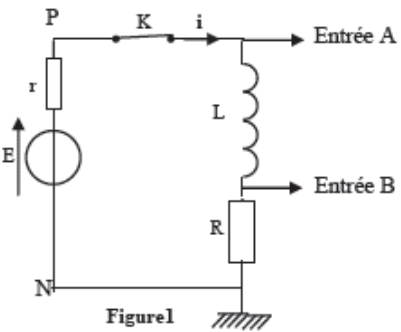
\includegraphics[width=0.22\textwidth]{./img/img03.png}
	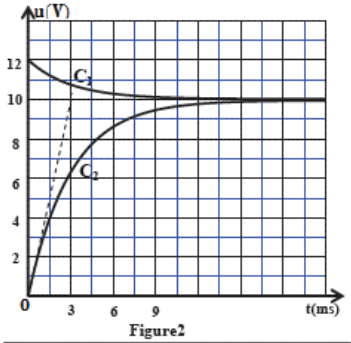
\includegraphics[width=0.25\textwidth]{./img/img04.png}
  \end{center}
\end{wrapfigure}
On réalise le circuit électrique, schématisé sur la figure 1, qui comporte : 
	\begin{itemize}
		\item  Un générateur de tension de f.e.m. $E=12V$
		\item  Une bobine d’inductance L et de résistance négligeable ;
		\item  Deux conducteurs ohmiques de résistance $R = 40\Omega$
		\item  Un interrupteur K.

	\end{itemize}

On ferme l’interrupteur K à l’instant $t=0$. Avec un système d’acquisition informatisé, on enregistre les
courbes (C2) et (C1 ) représentant les tensions des voies A et B (voir figure2).

\begin{tabular}{c|l}	

	0,25 & \makecell[l]{\textbf{1. }Identifier la courbe qui représente la tension $u_R (t)$ et celle qui\\représente $u_{PN} (t)$.}\\
	0,25 & \makecell[l]{\textbf{2. }Déterminer la valeur de $I_P$ l’intensité du courant électrique en \\régime
permanent. }\\
	0,25 & \makecell[l]{\textbf{3. }Vérifier que la valeur de la résistance $r$ du conducteur ohmique  \\est $r=8\Omega$. }\\
	
	1 & \makecell[l]{\textbf{4. }Etablir l’équation différentielle régissant l’établissement du courant $i(t)$ dans le circuit.  }\\
	1 & \makecell[l]{\textbf{5. }Trouver les expressions de A et de $\tau$ en
fonction des paramètres du circuit pour
que \\l’expression $i(t) =A (1-e^{-\frac{t}{\tau}} )$, soit solution de
cette équation différentielle. }\\

	1 & \makecell[l]{\textbf{6. }Déterminer la valeur de la constante du temps $\tau$. }\\
	1 & \makecell[l]{\textbf{7. }En déduire la valeur de l’inductance L de la bobine. }\\
	1 & \makecell[l]{\textbf{8. }Trouver l’énergie E emmagasinée par la bobine à l’instant $t = \frac{\tau}{2}$. }\\
	1 & \makecell[l]{\textbf{9. }Montrer que l’expression de la tension $u_{AB}(t)$ s’écrit :$u_{AB}(t) = -\frac{L}{\alpha}. \frac{du_{NB}}{dt}$,Trouver \\l'expressions de $\alpha$. }\\
\end{tabular}




	%\vspace{0.5cm}
%\textbf{2. Injection locale d’une solution contenant du rhénium 186.
%Le produit injectable se présente sous la forme d’une solution contenue dans un flacon de volume $V_0= 10 mL$ ayant une activité $a_0 = 4.10^9Bq$ à la date $t=0$, c'est-à-dire à la sortie du laboratoire pharmaceutique.}
	%\begin{tabular}{c|l}

		%1 & \makecell[l]{\textbf{2.1 }Déterminer en jours la valeur de demi-vie $t_{1/2}$ du rhénium $_{75}^{186}Re$}\\

		%0,5 & \makecell[l]{\textbf{2.2 }Trouver, à l’instant $t_1 = 4,8jours$, le nombre $N_1$ de noyau de rhénium contenu dans le flacon.}\\

		%0,5 & \makecell[l]{\textbf{3.2 } À l’instant $t_1$ on prélève du flacon de volume $V_0 = 10mL$ une injection de volume V contenant \\$N = 3,65.10^{13}$ noyaux de rhénium 186, on l’injecte à un malade dans l’articulation de l’épaule, \\trouver la valeur de V.}\\
	%\end{tabular}


%\section*{Partie 2 :  Centrale nucléaire \dotfill(9pts)}
%Dans une centrale nucléaire, les noyaux d'uranium $^{235}_{92}U$ subissent la fission sous le choc d'un neutron
%lent. Un des nombreux processus possibles conduit à la formation d'un noyau de lanthane $^{144}_{57}La$ ,d'un noyau de brome $^{88}_{35}Br$ et  de plusieurs neutrons.

%\begin{tabular}{c|l}

 %1& \makecell[l]{\textbf{1. } Définissez l'énergie de liaison d'un noyau.}\\

 %1 & \makecell[l]{\textbf{2. } Donnez l'expression littérale qui permettra son calcul.}\\

 %1 & \makecell[l]{\textbf{3. } Calculez, en MeV, l'énergie de liaison d’un noyau $^{235}_{92}U$.}\\

 %1 & \makecell[l]{\textbf{4. } Calculez l’énergie de liaison par nucléon de ce noyau.}\\

 %1 & \makecell[l]{\textbf{5. } Ecrivez l’équation de la réaction de fission étudiée.}\\

 %1 & \makecell[l]{\textbf{6. } Exprimez l'énergie libérée par la fission d'un noyau $^{235}_{92}U$ en fonction des énergies de liaison par
%\\ nucléon du noyau père et des noyaux fils et calculez la valeur de cette énergie en MeV.}

 %\end{tabular}

%\textbf{7.  Dans le cœur de la centrale, de nombreuses autres réactions de fission du noyau $^{235}_{92}U$ se produisent. La perte de masse est, en moyenne, de 0,200 u par noyau.}


%\begin{tabular}{c|l}

	%1,5 & \makecell[l]{\textbf{7.1. } Calculez, en MeV, l'énergie moyenne libérée par la fission d’un noyau. Ce résultat est-il \\en concordance avec celui de la question 6 ?}\\

	%1,5 &\makecell[l]{\textbf{7.2. }Calculez, en joule, l'énergie moyenne libérée par une mole de noyaux $^{235}_{92}U$ } 

%\end{tabular}

%\textbf{Données :}
%\begin{itemize}
	%\item Célérité de la lumière dans le vide : $c = 2,998 . 10^8 m.s^{-1}$  
	%\item Masse du noyau d’uranium 235 : $m( ^{235}_{92}U) = 235,0134u$ 

	%\item Energies de liaison par nucléon : $E_l/A(^{144}_{57}La) = 8,28MeV/nucl$éon  ; $E_l/A(^{88}_{35}Br)$=$8,56MeV/nucl$éon
	%\item Constante d'Avogadro : $N_A = 6,02.10^{23} mol^{-1}$
	%\item $1u$ = $1,66055.10^{-27}Kg$ et $1eV = 1,602.10^{-19}J$
	%\item Masse d’un proton : $m(^1_1p) = 1,0073u$ ; Masse d’un neutron $m(^1_0n) = 1,0087u$
%\end{itemize}





\end{document}
